% !TEX root = main.tex

%%%%%%%%%%%%%%%%%%%%%%%%%%%%%%%%%%%%%%%%%%%%%%%%%%%%%%%%%%%%%%%%%%%%%%%%%%%%%%%%%%%%%%%%%%%%%%%%
\section{原理}
%%%%%%%%%%%%%%%%%%%%%%%%%%%%%%%%%%%%%%%%%%%%%%%%%%%%%%%%%%%%%%%%%%%%%%%%%%%%%%%%%%%%%%%%%%%%%%%%

\subsection{ソレノイドによる磁場}
図1のような半径$a$,長さ$b$の円筒ソレノイドによって中心軸上$(r = 0)$のP点に
作られる$B_z$は,単位長さあたりの巻数を$n$,ソレノイドに流れる電流を$I$とすると,
$$
B_z=\frac{\mu_0 n I}{2}(\cos \theta_2 - \cos \theta_1)
$$
であるから,ソレノイドのそう巻き数をN$(=nb)$,左側からP点までの距離を$z$とすると,
$$
\cos \theta_1 = \frac{z-b}{\sqrt[]{a^2+(z-b)^2}}\quad,\quad \cos \theta_2 = \frac{z}{\sqrt[]{a^2+z^2}}
$$
であるから,
$$
B_z=\frac{\mu_0 NI}{2} \{ \frac{z}{\sqrt[]{a^2+z^2}} + \frac{b-z}{\sqrt[]{a^2+(z-b)^2}} \}
$$
となる.
\begin{figure}[!ht]
    \centering
    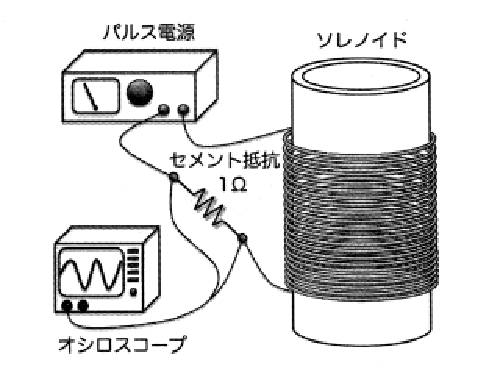
\includegraphics[scale=1]{figure1.pdf}
    \caption{有限長ソレノイド}
\end{figure}

\newpage

\subsection{磁気プローブ}
巻数$N$が1巻のコイルに鎖交する全磁束$\Phi$が時間変化すると,コイルの両端に,
$$
V_{c0}=-\frac{d\phi}{dt}
$$
の誘導電圧が現れる.このコイルの大きさが$\vec{B}$の空間変動に比べて十分小さければ,
コイルの断面積$S$上で$|\vec{B}|$が一定とみなすことができる.多くの場合,$N$の値
は$(\geq2)$であり,この時の全鎖交磁束は,
$$
\phi \simeq NBS
$$
であるから,
$$
V_{c0}=- \frac{d(NBS)}{dt}=-NS\frac{dB}{dt}
$$
と書ける.この式の右辺は$B$の時間微分の形になっているので,$B$を求めるためには
両辺を時間積分すれば良い.つまりコイル電圧$V_{c0}(t)$を時間積分することにより,
$$
B=-\frac{1}{NS} \int_{0}^{t} V_{c0}(t)dt
$$
として$B$の値を得ることができる.この方法を磁気プローブによる磁束密度測定法という.

\subsection{ロゴスキーコイルを用いた大電流測定}
アンペールの周回積分の法則より,任意の閉ループに沿った$B$の線積分はそのループと
鎖交する電流$i$の値を与え,ループの形状によらない.このことから,断面積$S$,
全巻き数$N$,長さが$l$のロゴスキーコイルが$i$を取り囲む形で置かれていると,
$$
\mu_0 i = \oint \vec{B} \cdot \vec{dl}
$$
という式が成り立つ.よって$i(t)$の作る磁束の時間変化によりロゴスキーコイルの両端
に現れる誘導電圧$V_e(t)$の関係は,
$$
i=-\frac{l}{\mu_0 NS}\int_{0}^{t} V_e(t)dt
$$
となる.また,電流路とロゴスキーコイルの相互インダクタンス$M$が既知の場合,$V_e$は,
$$
V_e=M\frac{dl}{dt}
$$
なので,
$$
i=\int_{0}^{t}\frac{1}{M}V_e(t)dt \simeq \frac{RC}{M}V_c
$$
としても求めることができる.